\documentclass[aspectratio=169]{beamer}
\usepackage{color}
\usepackage{tikz-cd}
\usepackage{smartdiagram}
\usepackage{appendix}
\usepackage{babel}
\usepackage{dsfont}
\usepackage{amsmath}
\usepackage{amssymb}
\usepackage{amsthm}
\usepackage{stmaryrd}
\usepackage{color}
\usepackage{array}
\usepackage{hyperref}
\usepackage{graphicx}
\usepackage{mathtools}
\usepackage{natbib}
\usepackage{tcolorbox}
\usepackage[bb=boondox]{mathalfa}

\theoremstyle{plain}
\newtheorem{thm}{Theorem}[section]
\newtheorem{lem}[thm]{Lemma}
\newtheorem{prop}[thm]{Proposition}
\newtheorem{coro}[thm]{Corollary}
\newtheorem{claim}{Claim}


\theoremstyle{definition}
\newtheorem{conj}{Conjecture}
\newtheorem{defi}{Definition}
\newtheorem{exercise}{\textbf{\textcolor{red}{Exercise}}}
\newtheorem{step}{Step}

\theoremstyle{remark}

\newtheorem*{rem}{Remark}

\newcommand{\homo}{\mathbf{Hom}}
\newcommand{\Max}{\mathbf{Max}}
\newcommand{\spec}{\mathbf{Spec}}
\newcommand{\spm}{\mathbf{Spec}_{max}}
\newcommand{\Frac}{\mathbf{Frac}}
\newcommand{\tr}{\mathrm{tr}}
\newcommand{\codim}{\mathrm{codim}}
\newcommand{\dif}{\text{d}}
\newcommand{\jac}{\textbf{Jac}}
\newcommand{\der}{\textbf{Der}}
\newcommand{\rank}{\text{rank}}
\newcommand{\sym}{\textbf{Sym}}
% 加导航条
\useoutertheme[width=2.9\baselineskip,right]{sidebar}
% 目录标数字
\setbeamertemplate{section in toc}[sections numbered]
% 无序列表用实心点
\setbeamertemplate{itemize item}{$\bullet$}
% 设置每页标题格式
\setbeamertemplate{frametitle}
  {\vspace{-0.5cm}
   \insertframetitle
   \vspace{-0.5cm}}
% 去掉下面没用的导航条
\setbeamertemplate{navigation symbols}{}
% 设置页脚格式
\makeatother
\setbeamertemplate{footline}
{
  \leavevmode%
  \hbox{%
  \begin{beamercolorbox}[wd=.4\paperwidth,ht=2.25ex,dp=1ex,center]{author in head/foot}%
    \usebeamerfont{author in head/foot}\insertshortauthor
  \end{beamercolorbox}

  \begin{beamercolorbox}[wd=.6\paperwidth,ht=2.25ex,dp=1ex,center]{title in head/foot}%
    \usebeamerfont{title in head/foot}\insertshorttitle\hspace*{13em}
    \insertframenumber{} / \inserttotalframenumber\hspace*{0ex}
  \end{beamercolorbox}}

  \vskip0pt%
}
%设置脚注字号
\setbeamerfont{footnote}{size=\zihao{7}}
\makeatletter


% 定义颜色
\definecolor{alizarin}{rgb}{0.82, 0.1, 0.26} % 红色
\definecolor{DarkFern}{HTML}{407428} % 绿色
%\colorlet{main}{DarkFern!100!white} % 第一种设置方法
\colorlet{main}{red!70!black} % 第二种设置方法
\definecolor{bistre}{rgb}{0.24, 0.17, 0.12} % 黑色
\definecolor{mygrey}{rgb}{0.52, 0.52, 0.51} % 灰色
%\colorlet{main}{green!50!black}
\colorlet{text}{bistre!100!white}

% 不同元素指定不同颜色,fg是本身颜色,bg是背景颜色,!num!改变数值提供渐变色
\setbeamercolor{title}{fg=main}
\setbeamercolor{frametitle}{fg=main}
\setbeamercolor{section in toc}{fg=text}
\setbeamercolor{normal text}{fg=text}
\setbeamercolor{block title}{fg=main,bg=mygrey!14!white}
\setbeamercolor{block body}{fg=black,bg=mygrey!10!white}
\setbeamercolor{qed symbol}{fg=main} % 证明结束后的框颜色
\setbeamercolor{math text}{fg=black}
% 设置页脚对应位置颜色
\setbeamercolor{author in head/foot}{fg=black, bg=mygrey!5!white}
\setbeamercolor{title in head/foot}{fg=black, bg=mygrey!5!white}
\setbeamercolor{structure}{fg=main, bg=mygrey!10!white} % 设置sidebar颜色

% 左右页间距的排版
\def\swidth{2.3cm}
\setbeamersize{sidebar width right=\swidth}
\setbeamersize{sidebar width left=\swidth}
\setbeamerfont{title in sidebar}{size=\scriptsize}
\setbeamerfont{section in sidebar}{size=\tiny}


%-------------------正文-------------------------%

\author{Deng Zhiyuan}
\title{Presentation in Zurich}
\subtitle{The equivalence of Godement-Jacquet and Jacquet-Langlands }
\date{\today}
\begin{document}

\frame[plain]{\titlepage}

\begin{frame}{Deng Zhiyuan}
    Deng Zhiyuan, from China, currently in Paris
    \begin{enumerate}
        \item[*] Undergraduate in Harbin Institute of Technology, 2017-2021: Mathematics and applied mathematics
        \item[*] Master 2 program in Aix-Marseille university, 2021-2022: Representation theory and Langlands program
    \end{enumerate}
\end{frame}
\begin{frame}{Awards/scholarships}
    \begin{enumerate}
        \item China Scholarship Council four years PhD funding for vertex operator algebra and quantum field theory  with Prof. Simon Wood at Cardiff University (Given up due to personal situation) (2021);
        \item S-T Yau mathematics contest silver medal (2020)
        \item Chinese college student mathematics contest bronze medal (2020)
        \item Prospective student of HIT (2019)
        

    \end{enumerate}
\end{frame}
\begin{frame}{Dissertations/other thesis}
    \begin{enumerate}
        \item[*] Freshman-Sophomore project advised by Prof. Niu Ben: Bifurcation  theory and ordinary differential equation (Predator-Prey model with infectious disease);
        \item[*] Undergraduate dissertation advised by Prof. Pi Qinghua: Reading project of representation theory of $GL(n, F)$, when $F$ is a non-Archimedean local field.
        \item[*] Master 2 dissertation advised by Prof. Farrell Brumley: The equivalence of Godement-Jacquet and Jacquet-Langlands $L$-function (Gal Dor's method \cite{dor2020exotic})
        \item[*] Current project advised by Prof. Farrell Brumley: Weyl's law with power saving error term with Finis-Lapid's method for $SL(2,\mathbb{Z})$ \cite{finis2021remainder}
    \end{enumerate}
\end{frame}
\begin{frame}{Research Interest/ Key words of dissertation/ thesis}
    \begin{itemize}
        \item Langlands program:
        \begin{itemize}
            \item Automorphic forms and $L$ functions (integral represenstation of $L$ function)
            \item Representation theory: (Local) theta correspondence, models (Whittaker) 
        \end{itemize}
        \item Trace formula:
        \begin{itemize}
            \item $GL_{2}$ trace formula with Hecke operators: Classical one from Hejhal, Strombergsson, Adelic: Jacquet-Langlands
            \item The application to Wely's law with fine error term (Selberg, Finis-Lapid)
        \end{itemize}
    \end{itemize}
\end{frame}

\begin{frame}
\frametitle{Content of the presentation}
\tableofcontents
\end{frame}


\section{The equivalence of Godement-Jacquet and Jacquet-Langlands }
\subsection{Classical Theory of Godement-Jacquet and Jacquet-Langlands}


\begin{frame}{Notations}
\begin{enumerate}
    \item     $F$ non-Archimedean  local field;
    \item  $G=GL_{2}(F)$
    \item $(\pi, V)$ representation of $G$;
    \item $(\tilde{\pi}, \widetilde{V})$ contragredient representation of $(\pi, V)$, in which $\widetilde{V}$ is the space of linear functional of $V$. And $\tilde{\pi}$ is defined as $\tilde{\pi}(g)\tilde{v}:=\tilde{v}\circ \pi(g)^{-1}$. And denote $<v,\tilde{v}>=\tilde{v}(v)$.
\end{enumerate}
\begin{rem}
The method by Gal Dor works for global field and $GL_{n}$ as well. But my master thesis only concentrates on local field. 
\end{rem}
\end{frame}
\begin{frame}
\frametitle{Riemann zeta function and L-function}
Riemann zeta function $\zeta(s)=\sum_{n\geq 1} \frac{1}{n^{s}},\ Re(s)>1$.  

\vspace{0.5 cm}

$L$-function is the generalization of Riemann zeta function.

\vspace{0.5 cm}

And $L$-functions are mysterious. Mainly we are interested in three properties:
\begin{enumerate}
    \item Analytic continuation;
    \item Functional equation;
    \item Location of zeros and values at special points;
\end{enumerate}
\end{frame}

\begin{frame}{The analytic theorem for Riemann zeta function}
    Let us recall the main analytic properties of the Riemann zeta function:
  
   \begin{thm}
   $\zeta(s)$ extends meromorphically to $\mathbb{C}$, with a simple pole $s=1$. It satisfies the functional equation 
   \begin{equation*}
       Z(s)=Z(1-s),\ \ \ \ \text{where}\  Z(s)=\pi^{-s/2}\Gamma(s/2)\zeta(s)
   \end{equation*}
   \end{thm}

\end{frame}
\begin{frame}{Hecke L-function}
    Hecke $L$-function means $L$-function extended by modular forms.
    
    \vspace{0.5 cm}
    
    A modular form is a holomorphic function defined on upper half plane with nice symmetry, which can be written as Fourier expansion $f(z)=\sum_{n \geq 0}a_{n}e^{2\pi inz}$. 
    
    \vspace{0.5 cm}
    
    Then here is the Hecke $L$-function: $L(f,s)= \sum_{n\geq 0}\frac{a_{n}}{n^{s}}$.
\end{frame}
\begin{frame}{Jacquet-Langlands L-function}
    The theory using classical language of modular form by Hecke was given an adelic and local interpretation by Jacquet and Langlands.
    
    \vspace{0.5 cm}
    
    The Jacquet-Langlands zeta integral:
    \begin{equation*}
        Z_{JL}(\phi,s)=\int_{ F^{\times}}\phi(y)|y|^{s-\frac{1}{2}}\dif^{\times}y 
    \end{equation*}
    in which $\phi\in \mathcal{K}(V)\cong V$, which is the only ingredient to construct the zeta integral.
\end{frame}
\begin{frame}
\frametitle{Kirillov model}
$\mathcal{K}(V)$ is the Kirillov model of the representation $(\pi,  V)$. 

\vspace{0.5 cm}

The model means an explicit realization of the abstract representation.

\vspace{0.5 cm}

Later the Schr\"odinger model means the same thing.
\end{frame}
\begin{frame}{Iwasawa-Tate L-function}
    The functional equation of $L$-function with Hecke character $L(s,\chi)$ is first proved by Hecke using the explicit theta function $\theta(t)=\sum_{n\in\mathbb{Z}}e^{-\pi n^{2} t}$.
    
    \vspace{0.5cm}
    
    Tate removed the need for any special functions. Iwasawa independently developed this theory as well but without an analog of the local theory in Tate's thesis.
\end{frame}
\begin{frame}{Godement-Jacquet L-function}
Iwasawa–Tate theory was extended to the general linear group $GL(n)$ over an algebraic number field and automorphic representations of its adelic group by Godement and Jacquet. 

\vspace{0.5 cm}

Tate's thesis can be viewed as the $GL(1)$ case of the work by Godement–Jacquet.
\end{frame}
\begin{frame}{Godement-Jacquet zeta integral}
    Godement-Jacquet zeta integral:
    \begin{equation*}
        Z_{GJ}=\int_{GL_{2}(F)}\Phi(g)\beta(g)|\det(g)|^{s+\frac{1}{2}}\dif^{\times}g
    \end{equation*}
    in which 
    \begin{enumerate}
     \item $\Phi\in \mathcal{S}(M_{2}(F))$ is a Bruhat-Schwartz function. 
        \item $\beta(g)=<\pi(g)v,\tilde{v}>$ is a matrix coefficient;
       
    \end{enumerate}
    
    So the space of ingredients to construct Godement-Jacquet $L$-function is $V\otimes \mathcal{S}(M_{2}(F))\otimes \widetilde{V}$. 
\end{frame}
\begin{frame}{Zeta integral}
    Zeta integral is a \textbf{machine/factory} to produce $L$-function. We put some ingredients into our machines (zeta integral), then we get our $L$-functions as the  results. 
    
    \vspace{0.5 cm}
    
    Choose a nice test function then calculate Godement-Jacquet zeta integral and Jacquet-Langlands zeta integral, which gives the same $L$-function. This is already well-known.
    
    \vspace{0.5 cm}
    
    Now we want a more conceptual and natural way to understand the equivalence to build $L$-functions.
\end{frame}
\subsection{Equivalence between two constructions}
\begin{frame}{Philosophy of proof}
    In one sentence: we want to understand those two machines (zeta integrals), rather than only care for the result ($L$-function).
    \begin{figure}
        \centering
        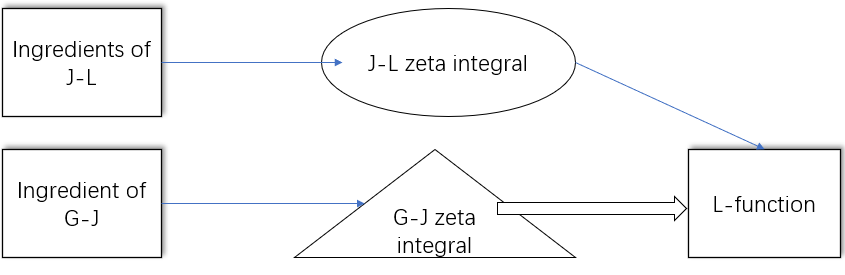
\includegraphics[scale= 0.37]{machine.png}
        \label{fig.machine}
    \end{figure}
    \vspace{0.3 cm}
    
    \textbf{Metaphor}:
\begin{center}
    \begin{tikzcd}
vector\ space \arrow[r, dashed] &  & zeta\ integrals
\end{tikzcd}
\begin{tikzcd}
basis \arrow[r, dashed]         &  & L-functions   
\end{tikzcd}
\end{center}
\end{frame}

\begin{frame}
\frametitle{The Philosophy of the proof}



The idea is to construct an isomorphism between two ingredient spaces with respect to calculation of zeta integrals for $L$-functions: $$\widetilde{V}\otimes_{G}\mathcal{S}(M_{2}(F))\otimes_{G} V\cong V.$$
\vspace{0.1 cm}

It's essential and more natural to know \textbf{how to build the machine} (zeta integral) rather than only care the product ($L$-function).
\end{frame}

\begin{frame}{G-modules}
    The isomorphism is between $G$-modules:
    \begin{enumerate}
        \item $\mathcal{K}(V)\cong V$ as a representation can be taken as a $G-module$.
        \item $\widetilde{V}\otimes_{G} V$ is a $G\times G$-module. By Schr\"odinger model, we construct $S(M_{2}(F))$ as a $G$-module as well, which introduced the third action into the space $\widetilde{V}\otimes_{G}S(M_{2}(F))\otimes_{G}V$. 
    \end{enumerate}
    
So we want to make $\widetilde{V}\otimes_{G}S(M_{2}(F))\otimes_{G}V$ a $G$-module then the isomorphism makes sense.
\end{frame}




\begin{frame}{The main theorem}
    There exists a third $G$-action on $Y=S(M_{2}(F))$, and this action is defined uniquely by two properties:
\begin{enumerate}
    \item This third action is commutative with the existing $G$-actions from the right and left;
    \item For every generic representation $(\pi, V)$, there is an isomorphism of $G$-modules:
    \begin{equation*}
        \nu:\widetilde{V}\otimes_{G}Y\otimes_{G}V\rightarrow V
    \end{equation*}
    \end{enumerate}
\end{frame}
\begin{frame}{Explicit the correspondence between G-J and J-L}

\begin{prop}
    Let $\Psi\otimes f\in \mathcal{S}(M_{2}(F))=Y$ be the function $\Psi(g)f(y)$. Then 
    \begin{equation*}
        Z_{JL}(\nu(\beta\otimes \Psi\otimes f),s)=Z_{GJ}(\beta,\Psi,s)\cdot \int_{F^{\times}}f(y)|y|^{s+\frac{1}{2}}d^{\times}y
    \end{equation*}
\end{prop}
This proposition gives an explicit correspondence between those two zeta integrals, in which $\nu$ is the isomorphism  above.
\end{frame}



\begin{frame}{The construction of the Middle Action}
The goal is to turn $S(M_{2}(F))$ into a Weil representation of a metapletic group. Then we use the action of this metapletic group to construct the desired middle action.  

\vspace{0.5 cm}


Then by using the Sch\"odinger model, we can calculate the explicit formula for our third action.
\end{frame}
\begin{frame}{Flow diagram of Proof}
    \begin{center}
        \begin{figure} 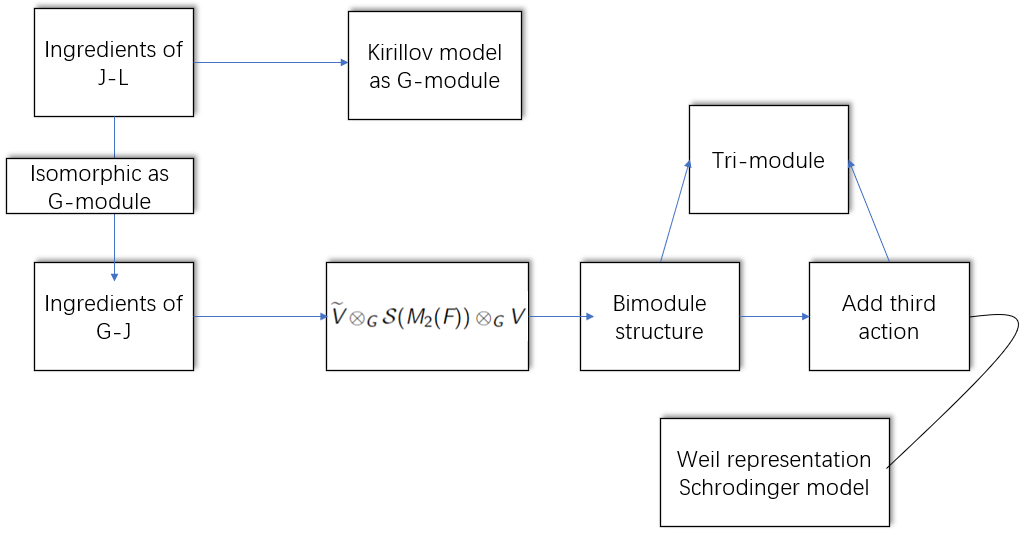
\includegraphics[scale=0.5]{proof.png}
            \label{png.proof}
        \end{figure}
    \end{center}
\end{frame}
\section{Current Project: Wely's law with power saving error term on $SL(2,\mathbb{Z})$}
\frame{\frametitle{Contents of the Thesis}\tableofcontents[currentsection]}
%\begin{frame}{Other thesis from undergraduate}
%My undergraduate dissertation is about %representation theory about $GL(n,F)$, when $F$ %is a non-archimedean local field. I studied the %$l$-structure by Bernstein and Zelevinski. The %main result is to present the dimension of %quotient space $E_{U,\theta^{-1}}$. However the %proof of the theme did not conclude in the %undergraduate thesis. And the information about %Whittaker model and Kirillov model. 
%\end{frame}
\begin{frame}{History of Wely's law}
    The famous metaphor is hearing the drum. If someones hears some sound (spectral side) from the drum, Then one can calculate the volume (geometry side) of the drum.
    
    \vspace{0.5 cm}
    
    Wely proved
    \begin{equation*}
        N(\lambda)=\frac{\textbf{Vol}(M)}{(4\pi)^{n/2}\Gamma(\frac{n}{2}+1)}\lambda^{n}+o(\lambda^{n}), \ \ \lambda\rightarrow\infty,
    \end{equation*}
    which can be taken an analog of  Rayleigh-Jeans law in physics.
    
\end{frame}
\begin{frame}{Wely's Law}
    The non-compact case is more complicated with one more term:
    \begin{equation*}
      M(\lambda)=-\frac{1}{4\pi}\int^{\lambda}_{-\lambda}\frac{\phi'}{\phi}(\frac{1}{2}+ir)\dif r,
    \end{equation*}
    in which 
    \begin{equation*}
      \phi(s)=\frac{\zeta^{*}(2s-1)}{\zeta^{*}(2s)},\ \ \zeta^{*}(s)=\pi^{-\frac{s}{2}}\Gamma(\frac{s}{2})\zeta(s).
    \end{equation*}
    $\phi(s)$ is the determinant of scattering matrix and described by Eisenstein series.
\end{frame}
\begin{frame}{Automorphic Wely's law}
    The project about automorphic Wely's law is the application of Selberg trace formula. 
    
    \begin{equation*}
    N(\lambda)+M(\lambda) \sim \frac{\text{Vol}(\Gamma\backslash \mathcal{H})}{4\pi}\lambda^{2},\ \ \ \lambda\rightarrow\infty    
    \end{equation*}
    
    
    This was first proved by Selberg. We are interested in $L^{2}_{cusp}$, and need to bound the contribution of $L^{2}_{cont}$ which is described by Eisenstein series. It can be done using the bound on Riemann zeta function.
\end{frame}
\begin{frame}{Development on this topic}
    For Maass forms on more general groups, this is difficult to generalize. 
    \begin{enumerate}
        \item[-$SL_{3}$] Steven Miller, with error term
        \item[-$SL_{n}$] Muller, no error term
        \item[-$SL_{n}$] Lapid-Muller, sharp error term
        \item[-$G$] Lindenstrauss-Venkatesh,  no error term
        \item[-$G$] Finis-Lapid+ Finis-Matz, power-saving error term
    \end{enumerate}
\end{frame}
\begin{frame}{Current Project}
    The idea of the current project is to use the new method of Finis-Lapid+Finis-Matz to explicit the proof for $SL_{2}(\mathbb{Z})$.
    
    \vspace{0.5cm}
    
    In their papers, they use amplification by Hecke operators but not Laplacian, which is the key to work with general groups. 
\end{frame}


% insert a reference frame before the 'thank you' frame ----------------------
\begin{frame}[allowframebreaks]
\frametitle{Citations}
\bibliographystyle{unsrt}
\bibliography{Langlands}
\end{frame}

% Insert a thank your frame ------------------------------------------------
\begin{frame}
\frametitle{Acknowledge}
\Huge{\centerline{Thank You!}}

\end{frame}
\end{document} 